\documentclass{article}
%\usepackage{geometry}
%\geometry{top = 1in, bottom = 1in, left = 1in, right = 1in}
\usepackage[top = 0.7in, bottom = 0.7in, left = 0.7in, right = 0.7in]{geometry}
\usepackage{amsmath,amssymb,amsthm,mathrsfs}
\usepackage{graphicx}
\usepackage{bm}
\usepackage{float}
\usepackage[font=footnotesize,labelfont=bf]{caption}
\usepackage{movie15}
\usepackage{hyperref}

\usepackage{fancyhdr}
\pagestyle{fancy}
\rhead{\footnotesize {february 2018} }
\chead{\footnotesize {Authors: } }
\lhead{\footnotesize {mesa/star/test\_suite/hb\_2M} }

\begin{document}
	
	\begin{center}
	  \begin{Large}
	    \textbf{HB 2M}\\
	  \end{Large}
	\end{center}

        This test is to show a 2 $M_\odot$ evolving on the Horizontal Branch, from ZACHeB (Zero Age Core Helium Burning) to TACHeB (Terminal Age Core Helium Burning). The convective boundary is determined using predictive mixing (see MESAIV paper), the Ledoux criterion, and semiconvection is turned on (but has no influence in this case since there is no composition gradient).\\
        
The inlists used to produce the TAMS (Terminal Age Main Sequence) model (inlist\_to\_TAMS) and the ZACHeB model (inlist\_to\_ZACHeB) are provided.\\

       The figures below show the evolution of the mass of the convective core and of the central helium abundance along the CHeB. In  figure \ref{fig:1} we show the effect of allowing (or not) the breathing pulses. These results were obtained using \texttt{max\_years\_for\_timestep=1d5} and \texttt{mesh\_delta\_coeff=0.5}.  In figure \ref{fig:2} we show the effect of using different values for \texttt{max\_years\_for\_timestep}. \\
 
 Note that in the test suite case we prevent the occurence of breathing pulses by using (\texttt{predictive\_avoid\_reversal = 'he4'}) and, for speed purposes, we use \texttt{max\_years\_for\_timestep=1d6}. The values used in the test suite case for the maximum allowed timestep and the mesh size do not produce converged models, as shown in (figure \ref{fig:2}). A smaller allowed maximum timestep should be used, and a convergence study should be done, when using this inlist for science purposes.\\

        
 
        \begin{figure}[H]
          \begin{minipage}[b]{0.5\linewidth}
	    \centering
	    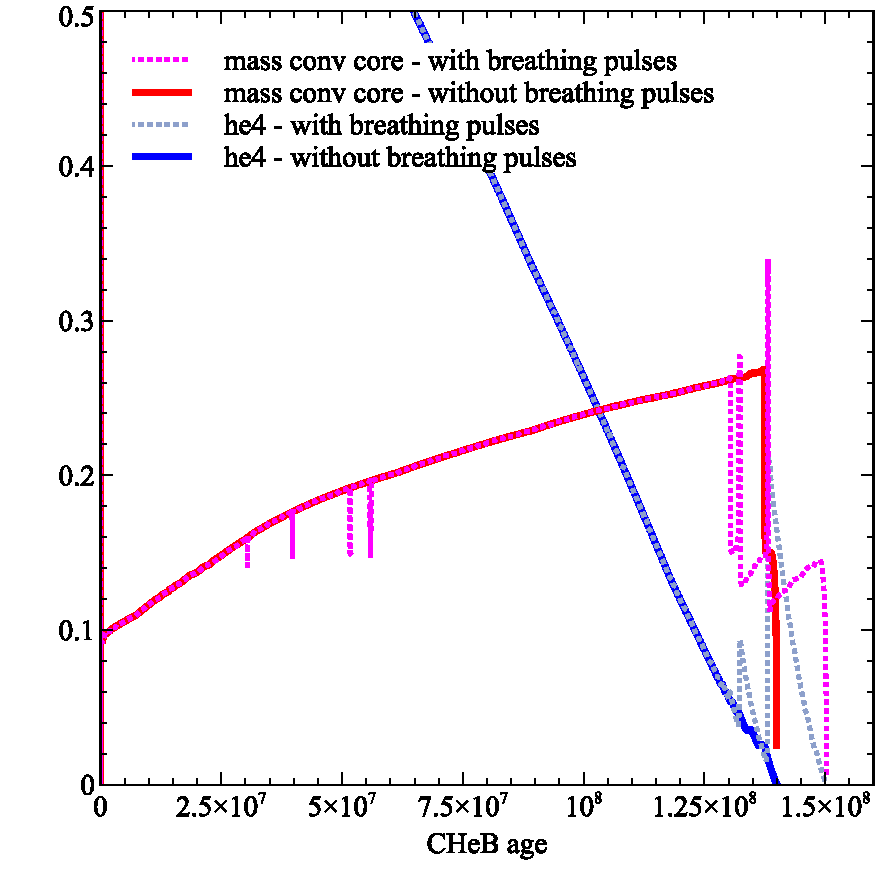
\includegraphics[width = 3.8in]{breathingpulses.pdf}
	    \caption{}
	    \label{fig:1}
          \end{minipage}
          \hspace{0cm}
          \begin{minipage}[b]{0.5\linewidth}
            \centering
            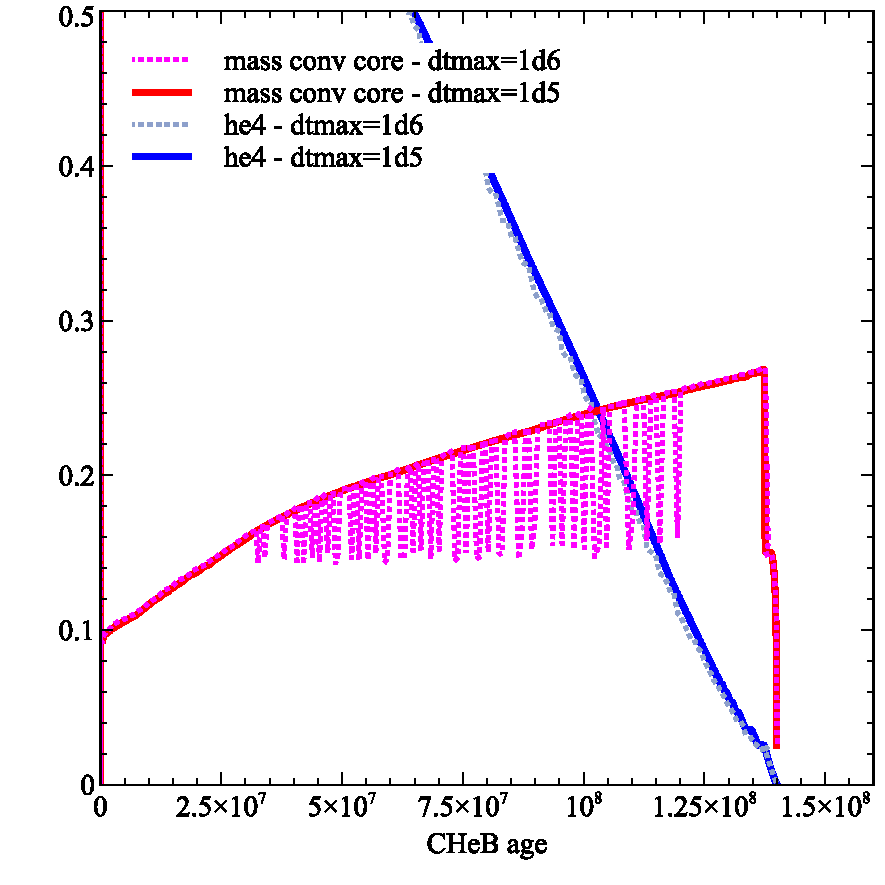
\includegraphics[width = 3.8in]{timestep.pdf}
            \caption{}
            \label{fig:2}
          \end{minipage}
	\end{figure}

        \pagebreak

        


\end{document}
